\documentclass[
  11pt,
  a4paper,
  % titlepage,
]{article}

\title{Data Structures, Algorithms and Databases}
\author{Martin de Spirlet}
\date{}

% Set document geometry
\usepackage[
  a4paper,
  margin = 1in,
  % showframe,
]{geometry} % Flexible and complete interface to document dimensions

% Set default font family to default sans-serif font
\renewcommand{\familydefault}{\sfdefault}

% Set default teletype font to Latin Modern Teletype
\renewcommand{\ttdefault}{lmtt}

\usepackage{amsmath} % AMS mathematical facilities for LaTeX
\usepackage{amssymb} % TeX fonts from the American Mathematical Society
\usepackage{booktabs} % Publication quality tables in LaTeX
\usepackage[labelfont=bf,labelsep=period]{caption}[2018/05/01] % Customising captions in floating environments
\usepackage[inline,shortlabels]{enumitem} % Control layout of itemize enumerate description
\usepackage{forest} % Drawing (linguistic) trees
\usepackage{graphicx} % Enhanced support for graphics
\usepackage{listings} % Typeset source code listings using LaTeX
\usepackage[skip=\glueexpr\baselineskip\relax]{parskip} % Layout with zero \parindent non-zero \parskip
\usepackage[onehalfspacing]{setspace} % Set space between lines % setspace must be loaded before hyperref
\usepackage{titlesec} % Select alternative section titles

\PassOptionsToPackage{hyphens}{url}\usepackage{hyperref} % Extensive support for hypertext in LaTeX % hyperref loaded by pdfx

% Set list parameters (using enumitem package)
\setlist{nosep}

% Define style for subtrees (using forest package)
% See https://tex.stackexchange.com/a/208792
\forestset{
  subtree/.style = {
    node format = {
      \noexpand\node [
        draw,
        shape = regular polygon,
        regular polygon sides = 3,
        inner sep = 0pt,
        outer sep = 0pt,
        \forestoption{node options},
        anchor = \forestoption{anchor},
      ] (\forestoption{name}) {\foresteoption{content format}};
    },
    child anchor = parent,
  },
}

% Load languages for listings (using package listings)
\lstloadlanguages{
  Java,
  SQL,
}

% Set listing parameters (using listings package)
\lstset{
  basicstyle = \ttfamily\fontseries{l}\selectfont,
  keywordstyle = \ttfamily\fontseries{b}\selectfont,
}

% Set section break command (using package titlesec)
\newcommand{\sectionbreak}{\clearpage}

% Define command for big-O notation
\newcommand{\bigo}[1]{O\!\left(#1\right)}

% Define command for improved overline in italic setting
\newcommand{\itol}[2][3]{{}\mkern#1mu\overline{\mkern-#1mu#2}}

% Increase penalty for widows and orphans (maximum 10000)
\widowpenalty = 10000
\clubpenalty = 10000

\begin{document}

\pagenumbering{gobble}

\maketitle

\vspace*{\fill}

\begin{table}[htp]
  \centering
  \begin{tabular}{rrl}
    \toprule
    Week & Unit & Title \\
    \midrule
     1 &  1 & Introduction and Entity Relationships \\
     2 &  2 & Functional Dependencies \\
     3 &  3 & Boyce-Codd Normal Form (BCNF) \\
     4 &  4 & Relational Algebra \\
     5 &  5 & Database Application Design \\
     7 &  6 & Linear and Binary Search \\
     8 &  7 & Binary Search Trees \\
     9 &  8 & AVL Trees \\
    10 &  9 & Graph Representations and Algorithms \\
    11 & 10 & Hash Tables \\
    \bottomrule
  \end{tabular}
\end{table}

\vspace*{\fill}
\addvspace{1in}

\clearpage

\pagenumbering{arabic}

\section{Introduction and Entity Relationships}
\subsection{The Benefits of Databases}

Databases provide
\begin{itemize}
  \item concurrent access for a large number of users,
  \item data integrity,
  \item high throughput and availability,
  \item fault tolerance, and
  \item the ability to store large amounts of structured data.
\end{itemize}

In addition, databases provide abstraction, and allow for the use of bespoke methods of access, such as structured query language (SQL).
Many database management systems (DBMS) make use of variations of SQL.

\subsection{SQL Tables}

SQL operates on \emph{tables}.
A table is the implementation of a \emph{relation} --- a theoretical construct with certain properties.
The rows of a table correspond to the \emph{tuples} of a relation.
The columns of a table correspond the the \emph{attributes} of a relation.

A relation is a \emph{set} of tuples.
Although a table may contain duplicate rows, a relation may not contain duplicate tuples.
Additionally, the way in which data is stored implies that tables are ordered in some way.
This is not the case for relations.

\begin{table}[htp]
  \centering
  \caption*{A table in SQL.}
  \begin{tabular}{rlr}
    \toprule
    id & name & mark \\
    \midrule
    1 & Alice & 90 \\
    2 & Bob & 80 \\
    3 & Charlotte & 70 \\
    4 & David & 60 \\
    \bottomrule
  \end{tabular}
\end{table}

The schema of a table is the logical definition of a table.
This includes the number of columns (attributes), their names and the type of information they store.

\subsection{Normalisation}

Storing all information in a single table leads to redundancy.
This can be avoided by \emph{normalising} tables --- linking information across multiple tables.

\subsection{Constraints}

SQL provides a way of imposing certain rules (\emph{constraints}) to tables.
Constraints include \texttt{NOT~NULL}, \texttt{UNIQUE}, \texttt{PRIMARY~KEY}, \texttt{FOREIGN~KEY}, \texttt{CHECK}, \texttt{DEFAULT} and \texttt{INDEX}.
A \emph{primary~key} is a set of attributes that uniquely identify a row.

\subsection{Database Design Goals}

A database design must
\begin{itemize}
  \item work within predefined business rules,
  \item ensure data consistency and throughput,
  \item contain all the required data, and
  \item ensure that the data remains readable despite these constraints.
\end{itemize}

Examples of business rules include
\begin{itemize}
  \item an order must be placed before it is shipped, and
  \item the timetables for a single student must not overlap.
\end{itemize}
These business rules can be implemented using database constraints.
Having the correct information with the required constraints constitutes \emph{data~quality}, which is critical to the smooth operation of an organisation.
Nevertheless, having all this required information in a database is not so useful if the database is too slow.
A balance must be struck between business requirements and throughput.

\subsection{Entity Relationship Diagrams}

\subsubsection{Crow's Feet Notation}

Entity relationship diagrams (ERDs) are a notation for database design.
There is no standard for (ERDs), but one popular family of notation is \emph{Crow's~Feet Notation}.

\subsubsection{Entities and Relationships}

Commonly, an entity is denoted by a rectangle.
An entity often represent nouns, such as objects or events.
The relationship between two entities is written on a line connecting them.
The relationship is usually a verb.
Thus, ERDs correspond to natural language.

\begin{figure}[htp]
  \centering
  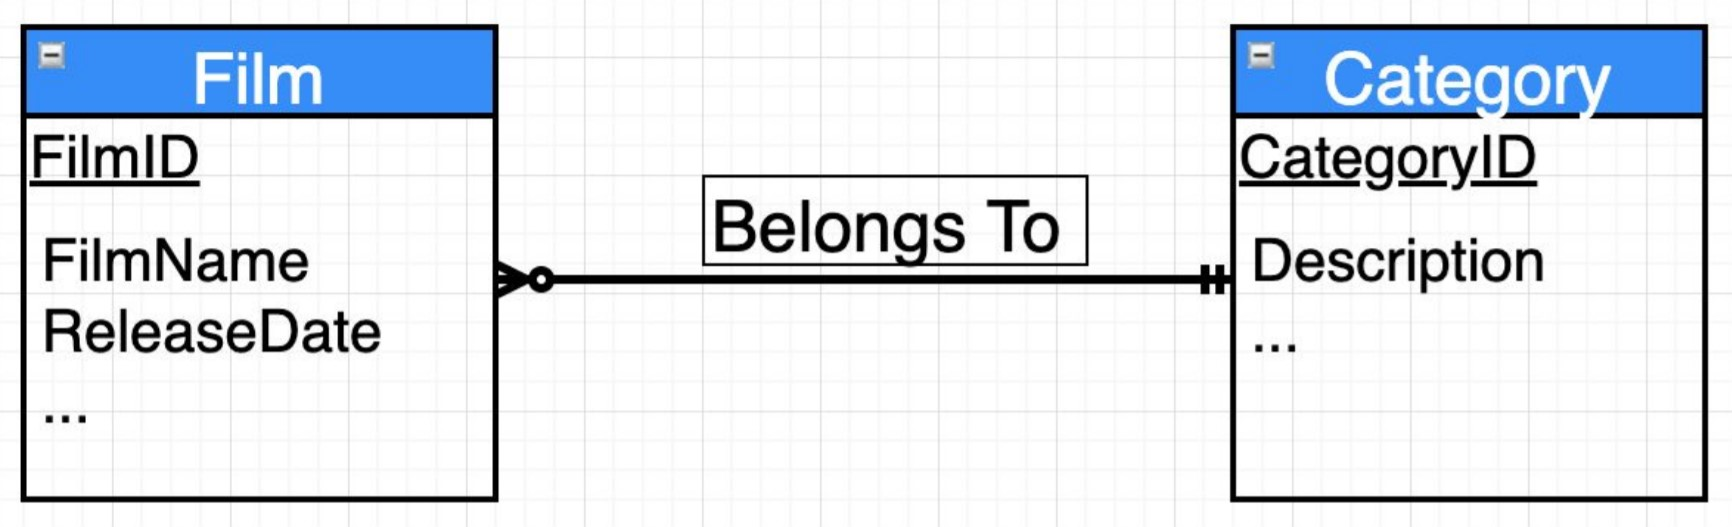
\includegraphics[width=0.75\textwidth]{unit-1/figures/er-diagram.jpg}
  \caption*{An entity relationship diagram.}
\end{figure}

The attributes of an entity are listed within its rectangle.
The primary key is underlined.

Relationships are named associations between entities.
Relationships provide associations in both directions.

\subsubsection{Cardinality}

\emph{Cardinality} provides a constraint on the number of instances of an entity that participate in a relationship.

\begin{figure}[htp]
  \centering
  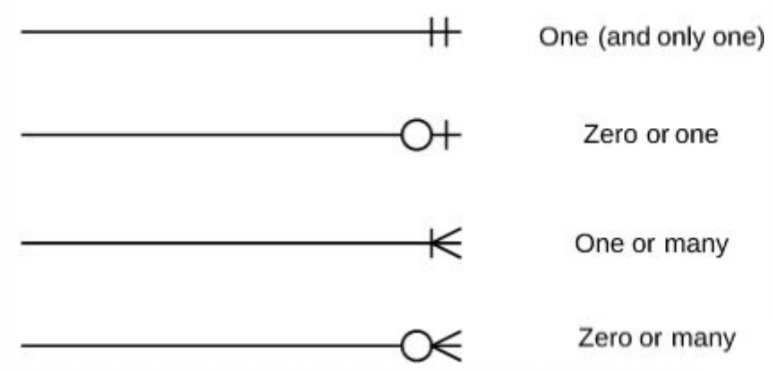
\includegraphics[width=0.6\textwidth]{unit-1/figures/cardinality-notation.jpg}
  \caption*{Cardinality notation.}
\end{figure}

\begin{table}[htp]
  \centering
  \caption*{Important cardinalities.}
  \begin{tabular}{ll}
    \toprule
    Name & Value \\
    \midrule
    Mandatory & Minimum cardinality \( \geq 1 \) \\ [1ex]
    Optional & Minimum cardinality \( = 0 \) \\ [1ex]
    Functional & Minimum cardinality \( = 1 \) \\ [1ex]
    \midrule
    One-to-one (1--1) & Maximum cardinality \( = 1 \) in both directions \\ [1ex]
    One-to-many (1--M) & Maximum cardinality \( = 1 \) in one direction \\
    & Maximum cardinality \( > 1 \) in the other direction \\ [1ex]
    Many-to-many (M--N) & Maximum cardinality \( > 1 \) in both directions \\
    \bottomrule
  \end{tabular}
\end{table}

\subsubsection{Foreign Keys and Weak Entities}

Relationships are translated to \emph{foreign~keys} in tables, except in the case of many-to-many relationships.

\emph{Weak~entities} are entities that do not have their own primary~key.
They must borrow attributes from other entities to form part or all of their primary~key.
Weak~entities are represented by rounded rectangles.
An underlined attribute of a weak~entity is not its primary key.
It is a key that is combined with the keys of one or more entities to provide a primary key.

\begin{figure}[htp]
  \centering
  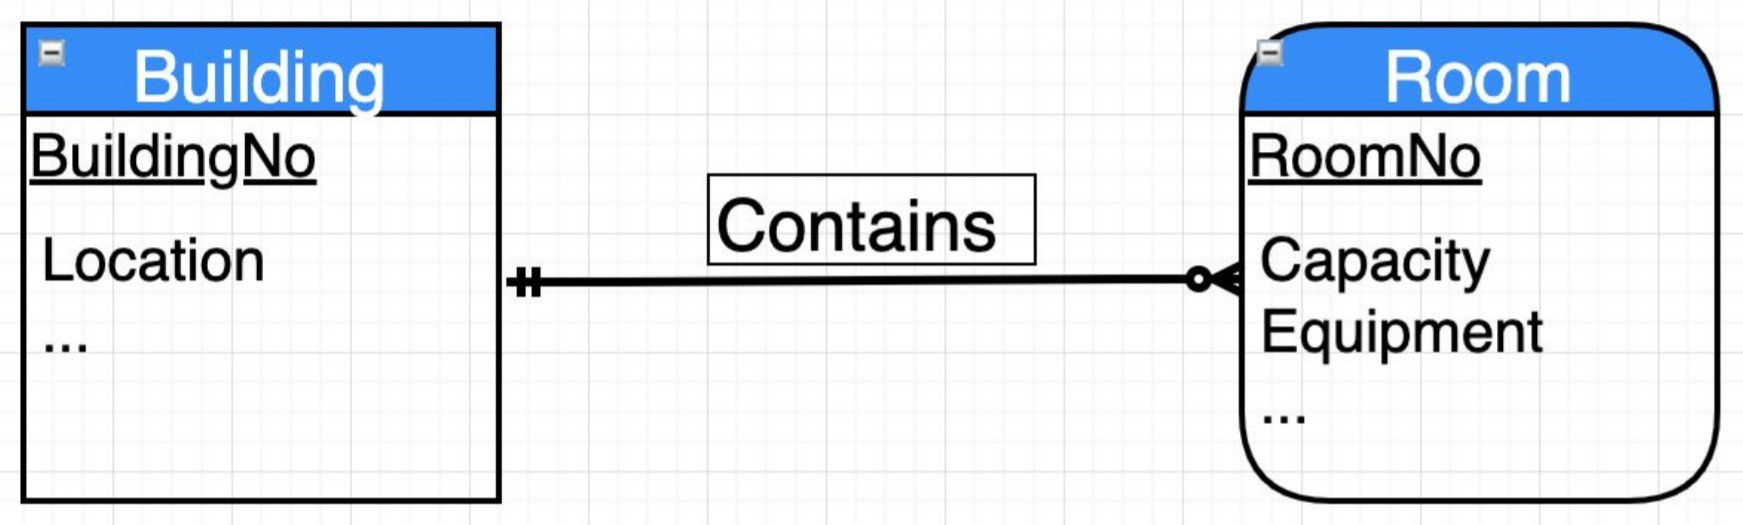
\includegraphics[width=0.75\textwidth]{unit-1/figures/weak-entity.jpg}
  \caption*{A weak entity relationship.}
\end{figure}

An \emph{identification relationship} provides one component of the primary key of a weak entity.
An \emph{identifying dependency} consists of one or more identification relationships that provide all of the primary key.
Sometimes an identification relationship and an identifying dependency are equivalent.

\subsubsection{Many-to-Many Relationships}

In a many-to-many relationship, the relationship itself can have attributes.
Theses attributes are listed below the relationship with an arrow pointing to them.

\begin{figure}[htp]
  \centering
  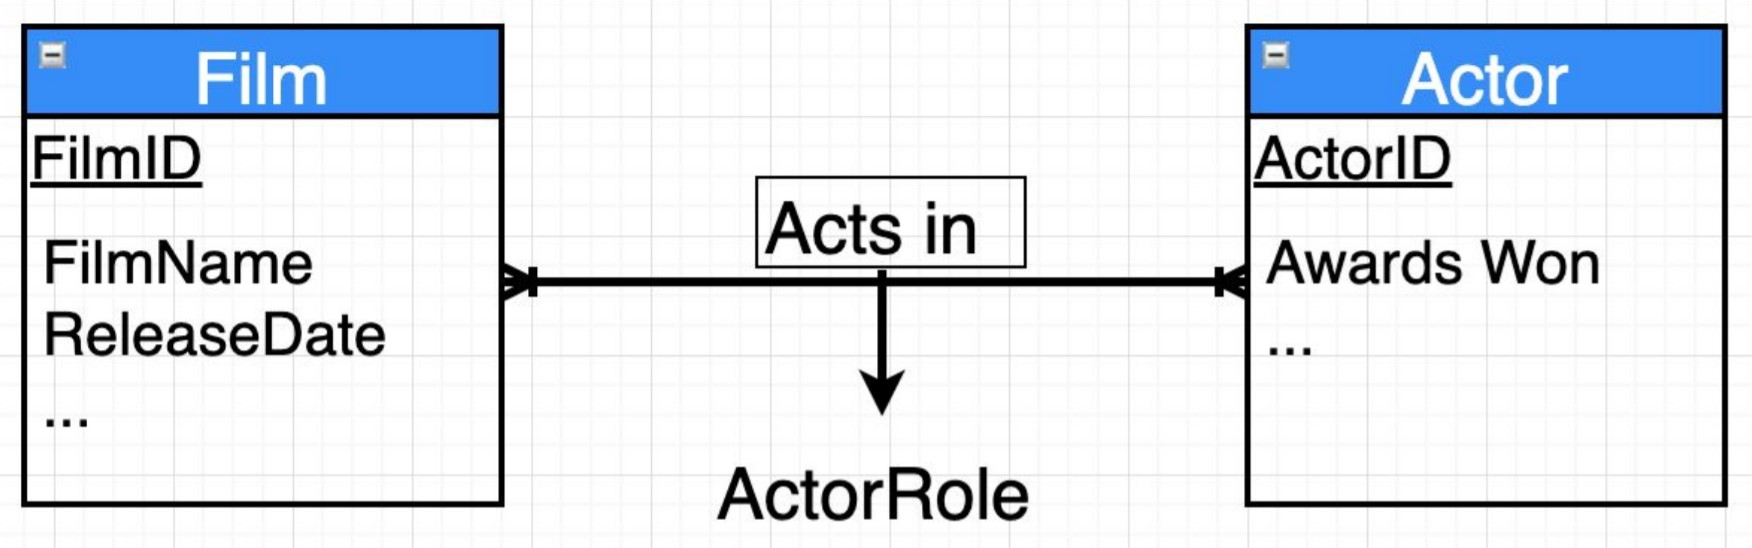
\includegraphics[width=0.75\textwidth]{unit-1/figures/relationship-attribute.jpg}
  \caption*{An attribute of a many-to-many relationship.}
\end{figure}

A many-to-many relationship can be replaced by an associate entity and two one-to-many relationships.

\begin{figure}[htp]
  \centering
  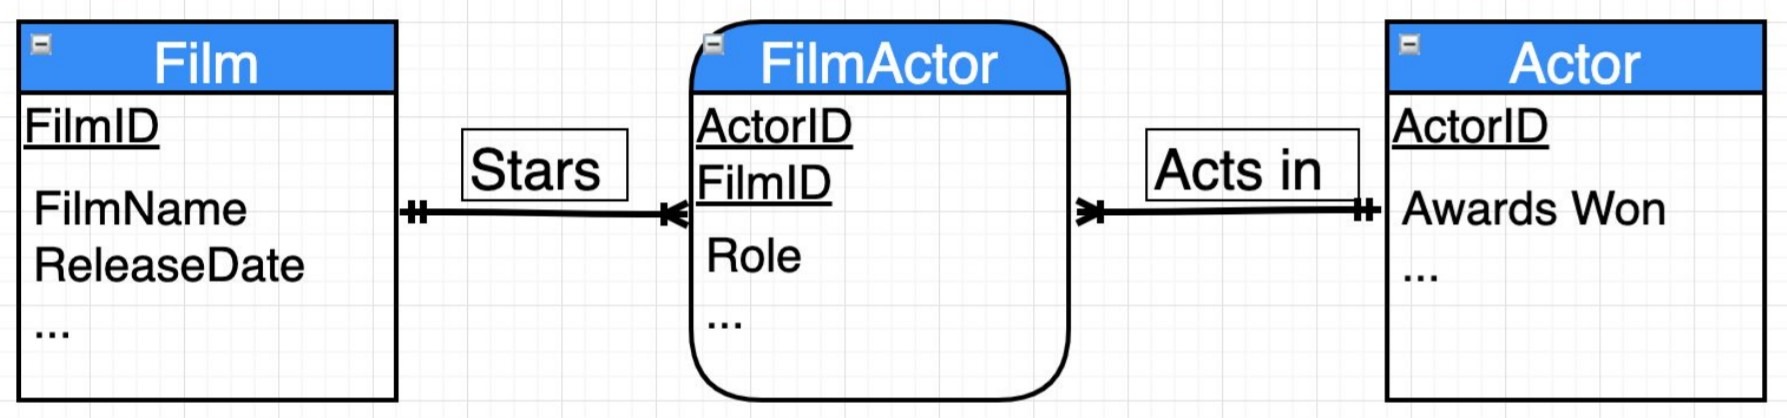
\includegraphics[width=\textwidth]{unit-1/figures/associate-entity.jpg}
  \caption*{An associate entity in a many-to-many relationship.}
\end{figure}

An associate entity provides additional information about the many-to-many relationship it implements.
By necessity, an associate entity is a weak entity that borrows the attributes of its primary~key from the entities between which it provides an association.

\subsubsection{\texorpdfstring{\( N \)}{N}-Way Relationships}

Sometimes --- though very rarely --- more than two entities are related to each other.
For example, a module may be taught by multiple lecturers, and a student is given a mark from each lecturer.
If it is only necessary to relate pairs of entities, such as which lecturers teach which modules, or which students are enrolled in which modules, an \( N \)-way relationship is not required.
If, however, it is necessary to store information associated with more than two entities, such as the mark given to a student from a lecturer for one section of a module, an \( N \)-way relationship is required.

\begin{figure}[htp]
  \centering
  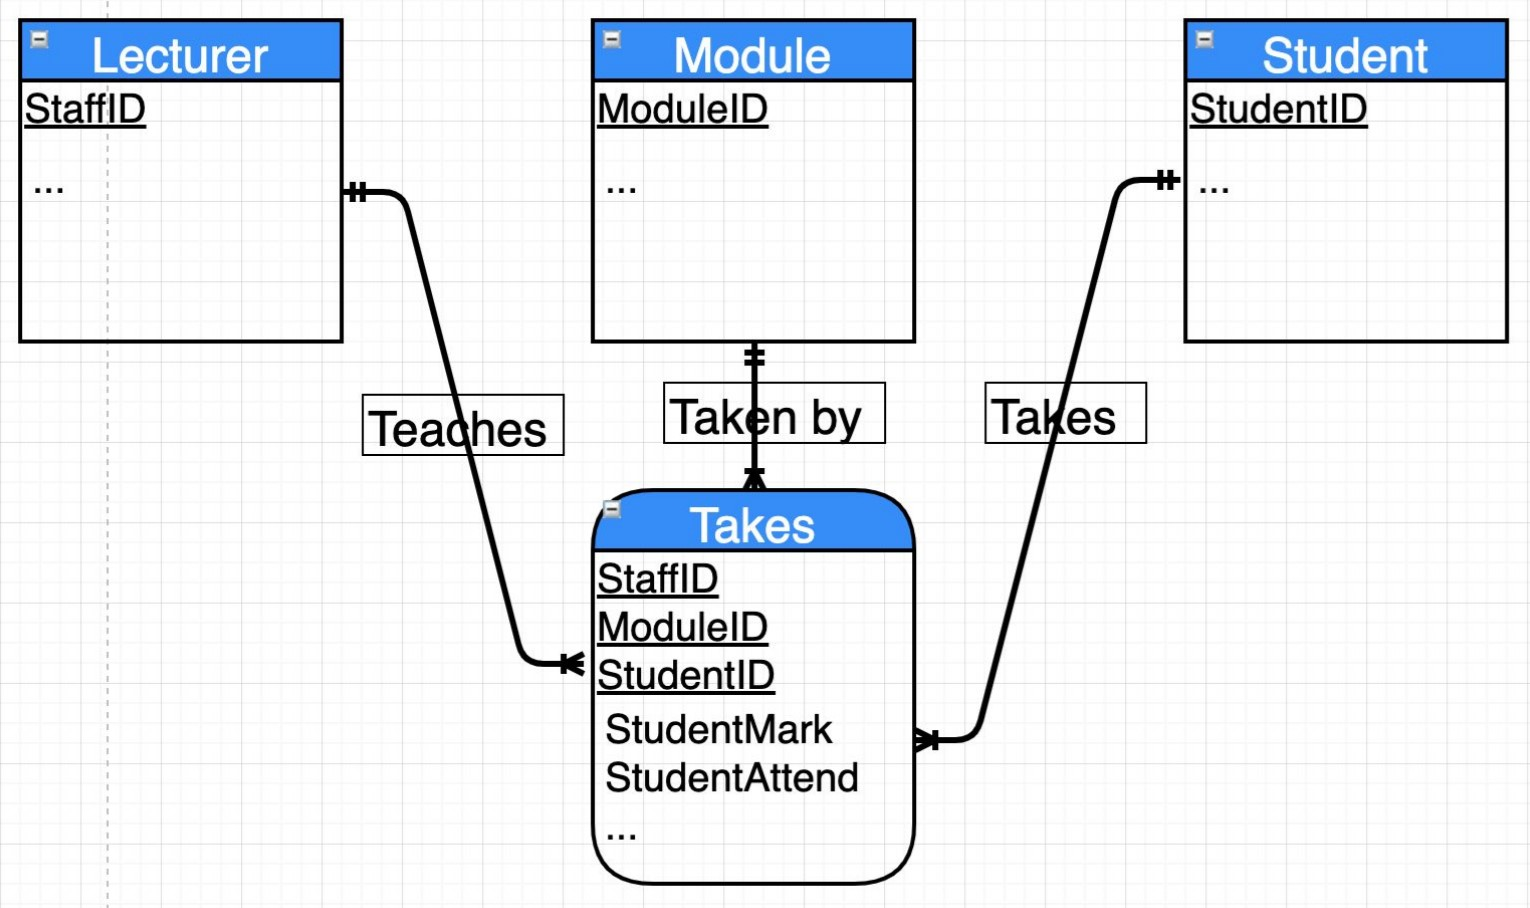
\includegraphics[width=\textwidth]{unit-1/figures/n-way-relationship.jpg}
  \caption*{An \( N \)-way relationship.}
\end{figure}

\subsubsection{Self-Identifying Relationships}

A \emph{self-identifying} (also \emph{self-referencing} or \emph{reflexive}) relationship is a relationship between an entity and itself.

\begin{figure}[htp]
  \centering
  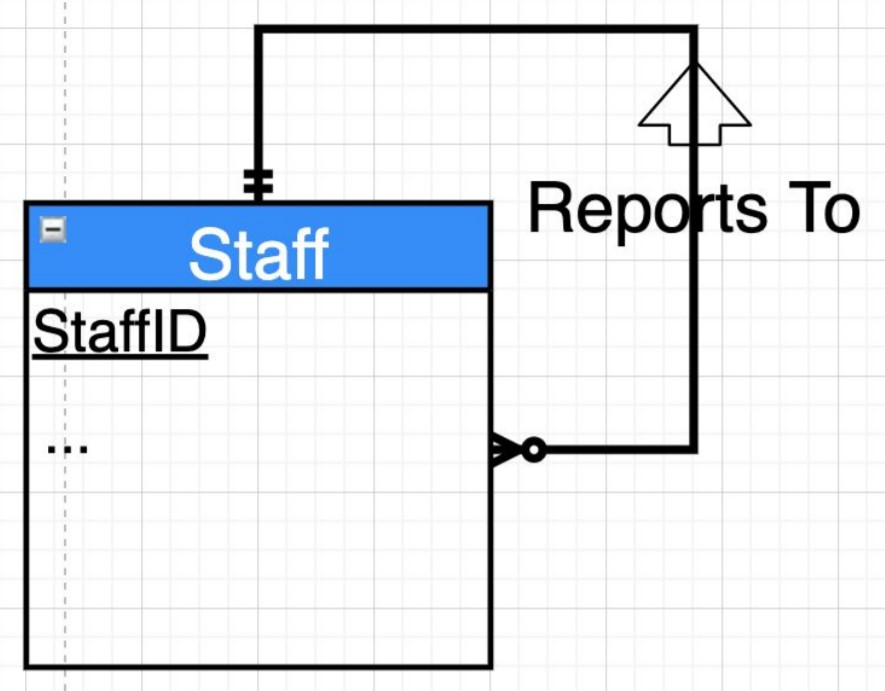
\includegraphics[width=0.4\textwidth]{unit-1/figures/self-identifying-relationship.jpg}
  \caption*{A self-identifying relationship.}
\end{figure}

All hierarchies are self-identifying relationships.
\begin{itemize}
  \item Biological classifications
  \item Organisational hierarchies
  \item Topic categories
\end{itemize}

In order to determine the cardinality of a self-identifying relationship, it is useful to draw an \emph{instance~diagram}.

\begin{figure}[htp]
  \centering
  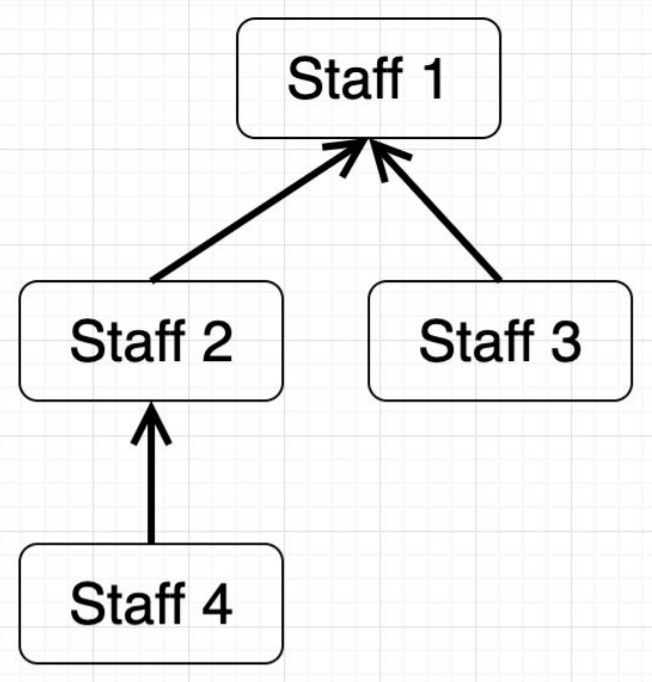
\includegraphics[width=0.3\textwidth]{unit-1/figures/instance-diagram.jpg}
  \caption*{An instance diagram of a self-identifying relationship.}
\end{figure}

A self-identifying relationship may require an associate entity, depending on its cardinality.
All self-identifying relationships can be translated to tables if many-to-many relationships are replaced by associate entities and one-to-many relationships.


\section{Functional Dependencies}
\subsection{Relational Design by Decomposition}

In its simplest form, all data could be stored in one large table with several columns.
The problem with this is that
\begin{itemize}
  \item the redundancy in repeated data will lead to a tremendous waste of space, and
  \item the throughput and availability of the data is diminished by the size of the table.
\end{itemize}

Instead, the large table is \emph{decomposed} into several smaller tables.

\subsection{Functional Dependency Notation}

\emph{Functional~dependencies} are a generalisation of keys.
The functional dependencies of a relation are based on knowledge of the real world.
All instances of the relation must adhere to its functional dependencies.

\begin{table}[htp]
  \centering
  \caption*{Attributes of the \emph{students} relation.}
  \begin{tabular}{llllllll}
    \toprule
    sID & sName & sAddress & fdUniCode & fdUniName & fdUniCity & fdUniMark & fdGrade \\
    \bottomrule
  \end{tabular}
\end{table}

Suppose that the `fdGrade' attribute of the students relation is based on the corresponding `fdMark'.
For example, a mark of 70 may map to a grade of A, and a mark of 60 may map to a grade of B\@.
It can be said that `fdGrade' is \emph{functionally~determined} by `fdMark', or `fdMark' \emph{functionally~determines} `fdGrade'.
In other words, any two tuples with the same `fdMark' must have the same `fdGrade'.
\begin{equation*}
  \text{fdMark} \rightarrow \text{fdGrade}
\end{equation*}

For every pair of tuples \( t \) and \( u \) that are elements of the student relation, the equality of the `fdMark' of both tuples implies the equality of the `fdGrade' of both tuples.
\begin{equation*}
  \forall\ t,u \in \text{students}: \quad t.\text{fdMark} = u.\text{fdMark} \implies t.\text{fdGrade} = u.\text{fdGrade}
\end{equation*}

In general, the functional dependency by which a set of attributes \( \itol{A} = \left\{ a_1, a_2, \ldots, a_m \right\} \) functionally determines a set of attributes \( \itol{B} = \left\{ b_1, b_2, \ldots, b_n \right\} \) in a relation \( R \) is defined as
\begin{equation*}
  \itol{A} \rightarrow \itol{B}
\end{equation*}
\begin{equation*}
  \forall\ t,u \in R: \quad t.\itol{A} = u.\itol{A} \implies t.\itol{B} = u.\itol{B}
\end{equation*}

\subsection{Interpreting Functional Dependencies}

The student~ID uniquely identifies a student; no two students can have the same ID\@.
\begin{equation*}
  \text{sID} \rightarrow \text{sName}
\end{equation*}

The student~ID uniquely identifies the registered address; a student cannot be registered under two addresses.
\begin{equation*}
  \text{sID} \rightarrow \text{sAddress}
\end{equation*}

The first~degree university~code uniquely identifies the name and city of the university; no two universities can have the same university~code.
\begin{equation*}
  \text{fdUniCode} \rightarrow \text{fdUniName}, \text{fdUniCity}
\end{equation*}

The name and city of a university uniquely identifies the university; no two universities in the same city can have the same name.
\begin{equation*}
  \text{fdUniName}, \text{fdUniCity} \rightarrow \text{fdUniCode}
\end{equation*}

The student~ID uniquely identifies the first~degree mark of the student with that ID; a student can only have one first~degree mark.
\begin{equation*}
  \text{sID} \rightarrow \text{fdMark}
\end{equation*}

The first~degree mark determines the first~degree grade; any two students with the same mark must have the same grade.
\begin{equation*}
  \text{fdMark} \rightarrow \text{fdGrade}
\end{equation*}

The student~ID uniquely identifies the first~degree grade of the student with that ID; a student can only have one first~degree grade.
\begin{equation*}
  \text{sID} \rightarrow \text{fdGrade}
\end{equation*}

\subsection{Functional Dependencies and Keys}

A key is a set of attributes that uniquely identifies a tuple.
If a set of attributes \( \itol{A} \) functionally determines all attributes of a relation \( R \) with no duplicates, then \( \itol{A} \) is a key of \( R \)\@.

\subsection{Types of Functional Dependency}

\subsubsection{Trivial Dependencies}

A functional dependency \( \itol{A} \rightarrow \itol{B} \) is said to be a \emph{trivial} functional dependency if \( \itol{B} \) is a subset of \( \itol{A} \).
\begin{equation*}
  \itol{A} \rightarrow \itol{B} \quad \text{is trivial if} \quad \itol{B} \subseteq \itol{A}
\end{equation*}

\subsubsection{Non-Trivial Dependencies}

A functional dependency \( \itol{A} \rightarrow \itol{B} \) is said to be a \emph{non-trivial} functional dependency if \( \itol{B} \) is \emph{not} a subset of \( \itol{A} \)\@.
\begin{equation*}
  \itol{A} \rightarrow \itol{B} \quad \text{is non-trivial if} \quad \itol{B} \nsubseteq \itol{A}
\end{equation*}

\subsubsection{Completely Non-Trivial Dependencies}

A functional dependency \( \itol{A} \rightarrow \itol{B} \) is said to be a \emph{completely non-trivial} functional dependency if \( \itol{A} \) and \( \itol{B} \) are disjoint, i.e.\ they share no common attributes --- their intersection is the empty set \( \varnothing \).
\begin{equation*}
  \itol{A} \rightarrow \itol{B} \quad \text{is completely non-trivial if} \quad \itol{A} \cap \itol{B} = \varnothing
\end{equation*}

\subsection{Rules of Functional Dependencies}

\subsubsection{The Splitting Rule}

The \emph{splitting rule} states that if
\begin{equation*}
  \itol{A} \rightarrow b_1, b_2, \ldots, b_n
\end{equation*}
then it follows that
\begin{equation*}
  \itol{A} \rightarrow b_1, \quad \itol{A} \rightarrow b_2, \quad \ldots, \quad \itol{A} \rightarrow b_n
\end{equation*}

\subsubsection{The Combining Rule}

The \emph{combining rule} states that if
\begin{equation*}
  \itol{A} \rightarrow b_1, \quad \itol{A} \rightarrow b_2, \quad \ldots, \quad \itol{A} \rightarrow b_n
\end{equation*}
then it follows that
\begin{equation*}
  \itol{A} \rightarrow b_1, b_2, \ldots, b_n
\end{equation*}

\subsubsection{The Transitive Rule}

The \emph{transitive rule} states that if
\begin{equation*}
  \itol{A} \rightarrow \itol{B} \quad \text{and} \quad \itol{B} \rightarrow \itol{C}
\end{equation*}
then it follows that
\begin{equation*}
  \itol{A} \rightarrow \itol{C}
\end{equation*}

\subsubsection{Trivial Dependency Rules}

If \( \itol{A} \rightarrow \itol{B} \) is a trivial dependency, then \( \itol{A} \) functionally determines the union of \( \itol{A} \) and \( \itol{B} \)\@.
\begin{equation*}
  \itol{B} \subseteq \itol{A} \implies \itol{A} \rightarrow \itol{A} \cup \itol{B}
\end{equation*}

If \( \itol{A} \rightarrow \itol{B} \) is a trivial dependency, then \( \itol{A} \) functionally determines the intersection of \( \itol{A} \) and \( \itol{B} \).
\begin{equation*}
  \itol{B} \subseteq \itol{A} \implies \itol{A} \rightarrow \itol{A} \cap \itol{B}
\end{equation*}

\subsection{Closure of Attributes}

The closure of a set of attributes \( \itol{A} \) in a relation is the set of all attributes \( \itol{B} \) such that \( \itol{A} \rightarrow \itol{B} \)\@.
The closure of \( \itol{A} \) is denoted by \( \itol{A}^{+} \)\@.
Since \( \itol{A} \) is a subset of itself, the closure of \( \itol{A} \) contains \( \itol{A} \)\@.
\begin{equation*}
  \itol{A} \subseteq \itol{A} \quad \therefore \quad \itol{A}^{+} \supseteq \itol{A}
\end{equation*}

In order to determine the closure of \( \itol{A} \),
\begin{enumerate}
  \item define a result set \( \itol{A}^{+} \) that initially contains all attributes of \( \itol{A} \), then
  \item repeating until there is no further change,
  \begin{enumerate}
    \item for all the (remaining) functional dependencies of the form \( \itol{X} \rightarrow \itol{Y} \),
    \begin{enumerate}
      \item if \( \itol{X} \) is a subset of the result set \( \itol{A}^{+} \),
      \begin{enumerate}
        \item add \( \itol{Y} \) to the result set \( \itol{A}^{+} \), and
        \item remove the functional dependency from the list of functional dependencies that remain to be considered.
      \end{enumerate}
    \end{enumerate}
  \end{enumerate}
  \item Finally, the result set \( \itol{A}^{+} \) should be the closure of \( \itol{A} \)\@.
\end{enumerate}

\subsection{Closure, Keys and Decomposition}

To check whether \( \itol{A} \) is a key of a relation \( R \), it is necessary to compute the closure of \( \itol{A} \)\@.
If the closure contains all attributes of \( R \), then \( \itol{A} \) is a key of \( R \)\@.

In general, to find all the keys for a relation \( R \), it is necessary to compute the closure of each and every subset \( \itol{A} \) of the attributes of \( R \)\@.
If the closure of the subset \( \itol{A} \) contains all attributes of \( R \), then \( \itol{A} \) is a key of \( R \)\@.
The problem can be simplified by noting that a superset of a key is itself a key.
Therefore, if a key \( \itol{A} \) is found, all supersets of \( \itol{A} \) can be marked as keys without having to compute their closures.

The purpose of decomposition is to find a minimal set of completely non-trivial functional dependencies such that all functional dependencies that hold on the original relation can be derived from this set.


\section{Boyce-Codd Normal Form (BCNF)}
\subsection{Natural Joins}

The \emph{natural~join} \( R \bowtie S \) of two relations \( R \) and \( S \) is the set of all combinations of the tuples of \( R \) and \( S \) whose common attributes are equal.

\begin{figure}[htp]
  \centering
  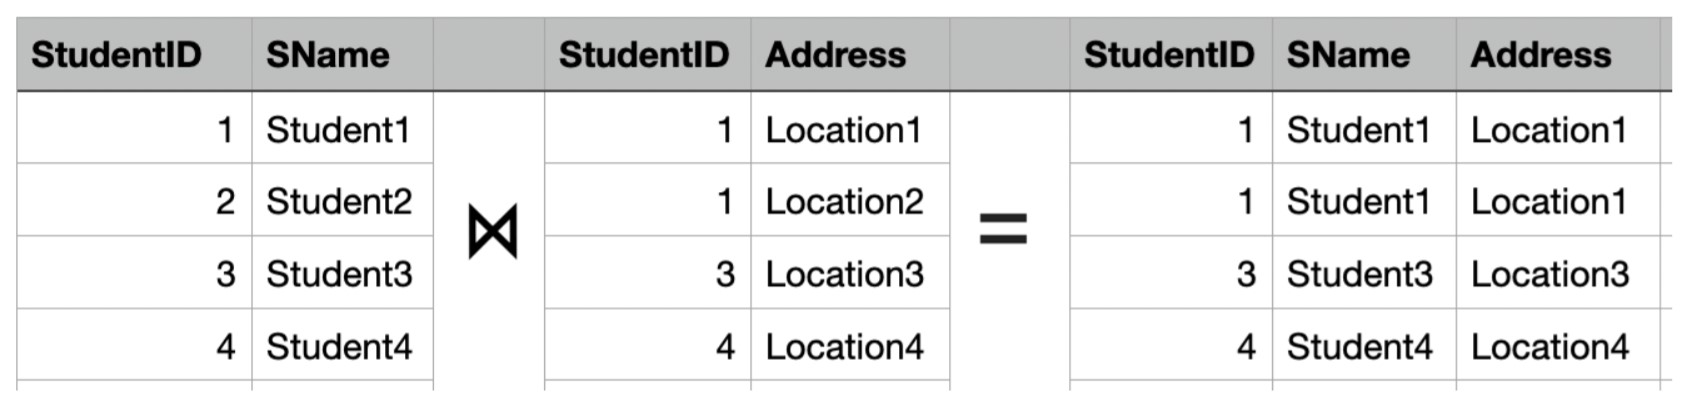
\includegraphics[width=0.8\textwidth]{unit-3/figures/natural-join.jpg}
  \caption*{The natural join of two relations.}
\end{figure}

\subsection{Decomposition of a Relation}

The decomposition of a relation \( R \), whose attributes are the set \( \itol{A} = \left\{ a_1, a_2, \ldots, a_m \right\} \), results in the creation of two new relations \( R_1 \) and \( R_2 \), whose attributes are the sets \( \itol{B} = \left\{ b_1, b_2, \ldots, b_n \right\} \) and \( \itol{C} = \left\{ c_1, c_2, \ldots, c_p \right\} \), respectively, such that \( R_1 \) and \( R_2 \) together contain all the attributes of \( R \), and the natural~join of \( R_1 \) and \( R_2 \) gives \( R \) exactly --- no more, no less.

Thus, all decomposed relations exhibit the following properties.
\begin{equation*}
  \itol{B} \cup \itol{C} = \itol{A}
\end{equation*}
\begin{equation*}
  R_1 \bowtie R_2 = R
\end{equation*}

\subsection{Identification of Boyce-Codd Normal Form (BCNF)}

A relation \( R \) is in \emph{Boyce-Codd Normal Form (BCNF)} if, and only if, for each of its functional dependencies \( \itol{A} \rightarrow \itol{B} \), \( \itol{A} \) is a key.

A functional dependency that causes a relation not to be in BCNF is called a \emph{BCNF~violation}.

\subsection{BCNF Decomposition Algorithm}

In order to decompose the relation \( R \),
\begin{enumerate}
  \item compute the keys of \( R \), then
  \item until all relations are in BCNF,
  \begin{enumerate}
    \item pick any of the problem relations \( R' \) with at least one functional dependency \( \itol{A} \rightarrow \itol{B} \) that violates BCNF (where \( \itol{A} \) is not a key),
    \item decompose it into two relations \( R_1\!\left( \itol{A}, \itol{B} \right) \) and \( R_2\!\left( \itol{A}, \text{rest} \right) \) --- discarding the original relation \( R' \), then
    \item compute the functional dependencies of \( R'_1 \) and \( R'_2 \), and
    \item compute the keys of \( R'_1 \) and \( R'_2 \).
  \end{enumerate}
  \item Finally, the remaining relations \( R' \) are the decomposition of the original relation \( R \).
\end{enumerate}

\begin{figure}[htp]
  \centering
  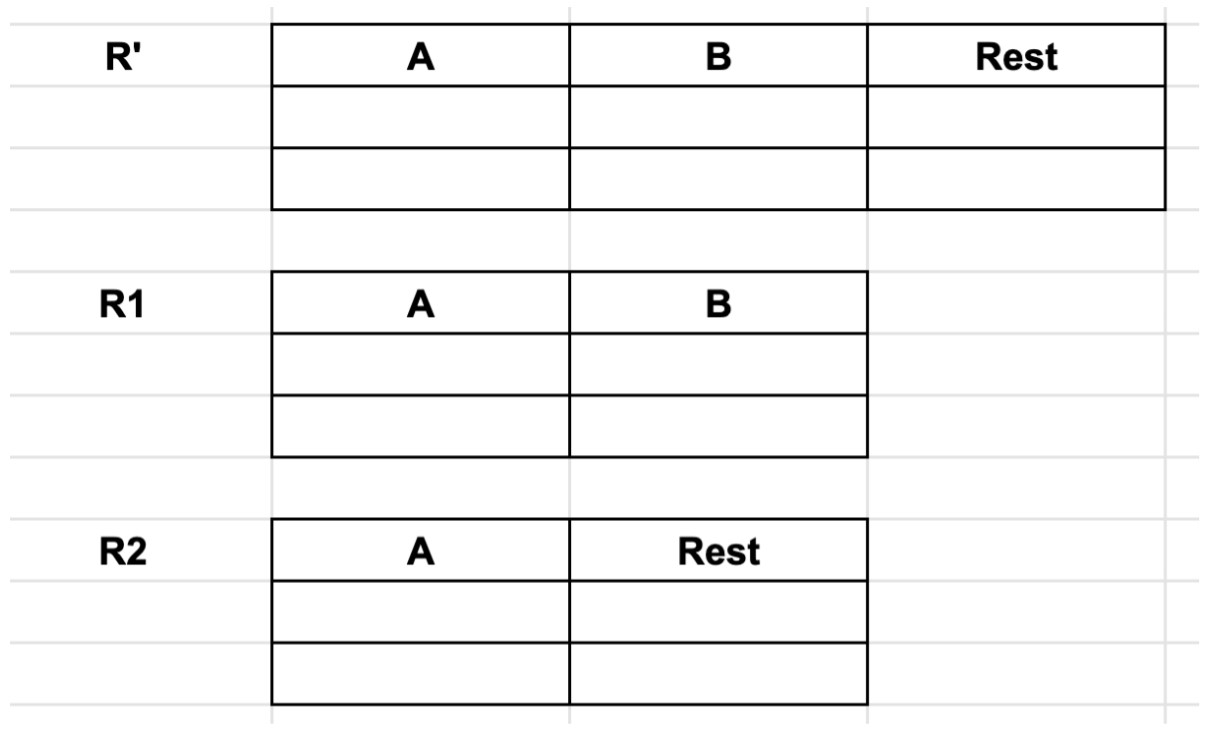
\includegraphics[width=0.6\textwidth]{unit-3/figures/decomposition.jpg}
  \caption*{Decomposition of a relation \( R'\!\left( \itol{A}, \itol{B}, \text{rest} \right) \) into \( R'_1\!\left( \itol{A}, \itol{B} \right) \) and \( R'_2\!\left( \itol{A}, \text{rest} \right) \).}
\end{figure}

The natural join of the decomposed relations \( R' \) is the original relation \( R \), and the union of the attributes of all \( R' \) is the set of attributes of \( R \).

BCNF provides the termination condition for decomposition.
A relation should be decomposed only if at least one of its functional dependencies is a BCNF~violation, and decomposition must continue until all relations are in BCNF, i.e. until there exists no relation with a functional dependency whose independent attributes are not a key.


\section{Relational Algebra}
\subsection{Background}

A database is a collection of relations (tables).
Relations consist of attributes (columns).
Data consists of tuples (rows).
A tuple has a value associated with each attribute.
A key is a set of one or more attributes that is unique to each tuple in a relation.

Each attribute has a domain (type) and every value has a type.
There is a special value \texttt{NULL} (undefined) that is a member of all domains.

The schema of a database includes the name, attributes and domains of every relation in the database.
An \emph{instance} of a database comprises the contents of its relations at a given point in time.

\emph{Relational algebra} is a formal language that underpins relational database query languages such as SQL\@.
A \emph{query} operates on one or more relations and returns a relation.
The simplest query in relational algebra is the name of a relation.
This simply returns a copy of the relation.

Relational algebra provides operators to
\begin{itemize}
  \item filter relations,
  \item slice relations, and
  \item combine relations.
\end{itemize}

\begin{table}[htp]
  \centering
  \caption*{The attributes of the \emph{students} relation.}
  \begin{tabular}{llll}
    \toprule
    sID & sName & sFirstDegree & sFDMark \\
    \bottomrule
  \end{tabular}
\end{table}

\begin{table}[htp]
  \centering
  \caption*{The attributes of the \emph{modules} relation.}
  \begin{tabular}{lll}
    \toprule
    mID & mName & mLecturer \\
    \bottomrule
  \end{tabular}
\end{table}

\begin{table}[htp]
  \centering
  \caption*{The attributes of the \emph{studentModules} relation.}
  \begin{tabular}{llll}
    \toprule
    sID & mID & caMark & examMark \\
    \bottomrule
  \end{tabular}
\end{table}

\subsection{Select Operation}

The \emph{select} operation \( \sigma_{\phi}\,R \) returns a new relation that comprises all tuples of a relation \( R \) for which a certain propositional formula \( \phi \) holds.
The propositional formula consists of atomic formulae and the logical operators \( \land \) (and), \( \lor \) (or) and \( \lnot \) (negation).

For example,
\begin{equation*}
  \sigma_{\text{sID}\,>\,1\ \land\ \text{sFDMark}\,>\,77}\,\text{students}
\end{equation*}
is equivalent to the SQL~query
\begin{lstlisting}[language={SQL}]
SELECT * FROM students WHERE sID > 1 AND sFDMark > 77;
\end{lstlisting}

\subsection{Project Operator}

The \emph{project} operation \( \pi_{a_1, \ldots, a_n}\,R \) returns a new relation that comprises all tuples of a relation \( R \) but with only a subset \( \left\{ a_1, \ldots, a_n \right\} \) of its attributes.

For example,
\begin{equation*}
  \pi_{\text{sID},\,\text{examMark}}\,\text{studentModules}
\end{equation*}
is equivalent to the SQL~query
\begin{lstlisting}[language={SQL}]
SELECT sID, examMark FROM studentModules;
\end{lstlisting}

\subsection{Chaining Operations}

Since these relational operations each act on a relation and return a relation, they can be chained.
For example,
\begin{equation*}
  \pi_{\text{sID},\,\text{examMark}}\!\left( \sigma_{\text{examMark}\,>\,70}\,\text{studentModules} \right)
\end{equation*}
is equivalent to the SQL~query
\begin{lstlisting}[language={SQL}]
SELECT sID, examMark FROM (
  SELECT * FROM studentModules WHERE examMark > 70
);
\end{lstlisting}

It is important to note that SQL tables are multisets and, therefore, allow duplicate rows.
Relations in relational algebra, however, are sets, and do not contain duplicate tuples.

\subsection{Cross Product or Cartesian Product}

The \emph{cross~product} or \emph{Cartesian~product} operator \( \times \) is used to combine two relations.
The result is a relation whose attributes are the union of the attributes of the two relations, and whose tuples are the cross~product of the tuples of the two relations.
\begin{equation*}
  R \times S
\end{equation*}

As a notational requirement, if the same attribute name exists in both relations, each corresponding attribute in the result is prefixed by the name of its source relation.

For example,
\begin{equation*}
  \text{students} \times \text{studentModules}
\end{equation*}
is equivalent to the SQL~query
\begin{lstlisting}[language={SQL}]
SELECT student.sID, sName, sFirstDegree, sFDMark,
       studentModules.sID, mID, caMark, examMark
FROM students, studentModules;
\end{lstlisting}

Typically, the cross~product is not useful unless it is filtered using a select operation.
For example,
\begin{equation*}
  \sigma_{\text{students.sID}\,=\,\text{studentModules.sID}}\!\left( \text{students} \times \text{studentModules} \right)
\end{equation*}
is equivalent to the SQL~query
\begin{lstlisting}[language={SQL}]
SELECT student.sID, sName, sFirstDegree, sFDMark,
       studentModules.sID mID, caMark, examMark
FROM students, studentModules
WHERE students.sID = studentModules.sID;
\end{lstlisting}

\subsection{Theta Join}

The \emph{Theta~join} operator \( \bowtie_{\Theta} \) performs the cross~product of two relations and selects all tuples of the result that satisfy the predicate \( \Theta \).
\begin{equation*}
  R \bowtie_{\Theta} S \equiv \sigma_{\Theta}\!\left( R \times S \right)
\end{equation*}
\begin{lstlisting}[language={SQL}]
SELECT * FROM R JOIN S ON <Theta>;
\end{lstlisting}

\subsection{Natural Join}

The \emph{natural~join} operator \( \bowtie \) performs the cross~product of two relations and selects all tuples of the result where each pair of attributes with the same name have the same value.
It then discards one attribute from each duplicate pair.
\begin{equation*}
  R \bowtie S \cong \sigma_{R.\itol{A}\,=\,S.\itol{A}}\!\left( R \times S \right)
\end{equation*}

For example,
\begin{equation*}
  \text{students} \bowtie \text{studentModules} \cong \sigma_{\text{students.sID}\,=\,\text{studentModules.sID}}\!\left( \text{students} \times \text{studentModules} \right)
\end{equation*}
is equivalent to the SQL~query
\begin{lstlisting}[language={SQL}]
SELECT * FROM students NATURAL JOIN studentModules;
\end{lstlisting}

The natural~join does not add expressive power to relational algebra since it can be expressed as a combination of projection, selection and cross~product.

\subsection{Rename Operator}

The \emph{rename} operation \( \rho_{S\left( b_1,\,\ldots,\,b_n \right)} R \) is used to rename a relation \( R \) and its attributes \( \left\{ a_1, \ldots, a_n \right\} \) to a relation \( S \) with attributes \( \left\{ b_1, \ldots, b_n \right\} \).

For example,
\begin{equation*}
  \rho_{S\left( b_1,\,\ldots,\,b_n \right)} R
\end{equation*}
is equivalent to the SQL~query
\begin{lstlisting}[language={SQL}]
SELECT a1 AS b1, ..., an AS bn FROM R AS S;
\end{lstlisting}

A relation can can be renamed without renaming its attributes using the following shorthand notation.
\begin{equation*}
  \rho_{S}\,R
\end{equation*}

As long as a relation has more than one attribute, all of its attributes can be renamed without renaming the relation using the following shorthand notation.
\begin{equation*}
  \rho_{b_1,\,\ldots,\,b_n}\,R
\end{equation*}

The rename operator adds expressive power to relational algebra as it is required in order to refer to specific attributes of a relation formed by a self~join.

\subsection{Self Join}

A \emph{self~join} is any type of join (cross~product, Theta~join or natural~join) whose two operands are the same relation.
In order to refer to specific attributes of a relation formed by a self~join, it is necessary to create renamed copies of the original relation before joining.

For example, a relation that describes pairs of modules taught by the same lecturer can be formed as follows.
The select operation discards tuples in which both modules are the same (\( \text{M1.mName} = \text{M2.mName} \)) or are reversed (\( \text{M1.mName} > \text{M2.mName} \)).
\begin{equation*}
  \begin{split}
    & \pi_{\text{M1.mName},\,\text{M2.mName}}\!\left(\right. \\
    & \quad \sigma_{\text{M1.mName}\,<\,\text{M2.mName}}\!\left(\right. \\
    & \quad \quad \rho_{\text{M1}\left( \text{M1.mID},\,\text{M1.mName},\,\text{mLecturer} \right)} \text{modules} \\
    & \quad \quad \quad \bowtie \\
    & \quad \quad \rho_{\text{M2}\left( \text{M2.mID},\,\text{M2.mName},\,\text{mLecturer} \right)} \text{modules} \\
    & \quad \left.\right) \\
    & \left.\right)
  \end{split}
\end{equation*}

\subsection{Set Operators}

The basic set operators are \emph{union} \( \cup \), \emph{difference} \( - \) and \emph{intersection} \( \cap \).
In relational algebra, these operators may only be applied to relations of the same schema.
In order to find the union of student names (`sName') and module names (`mName'), for example, it is necessary first to project only these attributes from their respective relations, and to give the attributes the same name.

The intersection operator does not add expressive power to relation algebra, as an intersection can be expressed as a combination of differences.
\begin{equation*}
  A \cap B \equiv A - \left( A - B \right)
\end{equation*}

Assuming two relations are of the same schema, their intersection is equivalent to their natural~join.
\begin{equation*}
  A \cap B \equiv A \bowtie B
\end{equation*}


\section{Database Application Design}
\subsection{Data Redundancy}

A relation is in \emph{first normal form} if each of its attributes holds only a single value for each tuple.
An attribute of a tuple may not hold an array or list of values, such as a string of comma-separated values.

A relation is in Boyce-Codd Normal Form (BCNF) if the set of dependent attributes of each of its functional dependencies is a key.
BCNF ensures that decomposed tables can be joined without loss of information, and that there is no redundancy in data.

While a policy of no redundancy is good for minimising the storage size of a database, it is not necessarily the best solution.
For example, data that are frequently accessed together may be split across multiple decomposed tables.
A join would be required every time these data are accessed.
This leads to
\begin{itemize}
  \item more complex queries and, therefore, a greater chance of an error that causes an incorrect result, and
  \item additional load on the system in order to perform the join.
\end{itemize}
Clearly, it is useful for some relations to include data redundancy so as to ensure that data frequently accessed together are available in the same table.
A compromise must be made between minimal storage size and minimal computation.

\subsection{Indices}

An \emph{index} is a persistent data structure that is used to improve the performance of a database management system (DBMS) when accessing tuples with a particular attribute value.
An index groups subsets of tuples in a relation according to a property of one of its attributes.
For example, tuples could be grouped according to the first character in an attribute `firstName'.
This increases the speed of data access, as only a subset of the tuples need to be searched for a particular value.

The author of a query does not need to use an index directly.
The query processor of the DBMS will automatically use an available index when appropriate.

An index can be created for any attribute in a database.
The creation of an index is computationally expensive, so only frequently queried attributes should be indexed.
Typically, an index is created as soon as sufficient queries have been made in order to determine the critical attributes.
Updating an index when a tuple is added to a relation is also computationally expensive.
Hence, indices are not created for highly dynamic tables.
An attribute is suitable for indexing if it appears often in \texttt{WHERE} or \texttt{JOIN ON} clauses.
It is possible to create a single index for multiple attributes that are compared in different ways.

The data structure used to implement an index is dependent on the type of attribute and the type of comparison made on it.
The two main data structures used as indices are \emph{hash~tables} and \emph{balanced~trees} (\emph{B-trees}).
A hash~table can only index attributes that are compared via equality, and can be searched in constant time \( \mathrm{O}\!\left( 1 \right) \).
A B-tree is used to index attributes that are compared via inequality relations (greater than or less than), and can be searched in logarithmic time \( \mathrm{O}\!\left( \log n \right) \).
Without an index, a relation can be searched in linear time \( \mathrm{O}\!\left( n \right) \).

Many DBMSs automatically create indices for primary keys.
It is assumed that the primary key will be used frequently in filter and join conditions.
Some DBMSs create indices for attributes that take unique values.
In order to improve the performance of a frequent join, the joined attributes of both relations must be indexed.

An index implicitly provides values of its attribute in sorted order, as this is useful for merge operations.
Attributes that are frequently sorted are suitable for indexing.

\subsection{Transactions}

\subsubsection{Consistency and Fault Tolerance}

\emph{Transactions} provide \emph{consistency} and \emph{fault tolerance} for database operations.
Consistency includes the enforcement of business constraints on data.
Fault tolerance includes limiting the extent of data loss when a failure occurs and avoiding irreparable damage to data.

There are many layers of data access in a database application.
A user calls upon an application for some data.
The application calls upon methods of the DBMS for the data.
The DBMS directly accesses the data to be returned.

All database statements are transactions.
Statements can be grouped to run as a transaction.
A transaction is executed either completely or not at all.

Transactions maintain the properties of \emph{isolation}, \emph{durability}, \emph{atomicity} and \emph{consistency}.
These properties are collectively known as \emph{ACID} and ensure that a system is both fault tolerant and consistent in terms of the operation of its transactions and its business requirements.

\subsubsection{Isolation}

\emph{Isolation} allows multiple clients working concurrently on a database to assume that they are the only client operating on the data.
A client does not have to worry about the operations performed by other clients.

Isolation is implemented using \emph{serialisability}.
Serialisable transactions may be interleaved so long as the end result would be equivalent to \emph{some} sequential execution of those transactions.
Serialisability does not guarantee that the result of interleaved transactions will be equivalent to a \emph{specific} order of execution.

\subsubsection{Durability}

\emph{Durability} ensures that if a failure occurs after the completion of a commit, the results and availability of previous transactions will not be affected.
Durability makes no guarantees on the state of changes made after the commit.

Durability is implemented using a log of all changes to the data.
This enables changes to be replayed over the original data in order to restore to any point in committed history.
For safety, the log must be stored separately from the data.

\subsubsection{Atomicity}

\emph{Atomicity} ensures that if a failure occurs before a commit is made, all transactions that were issued since the last commit are executed either in full or not at all.
No transaction is left partially executed due to a failure.
This is also implemented using  a log of all changes to the data.

The changes made by transactions that did not complete before the failure are undone via a \emph{rollback}.
A rollback can also be initiated by a client.

Transactions are usually \emph{blocking}, except in the case of interleaved serialisable transactions.
This means that when one transaction is working on a particular table, another transaction cannot work on that table.

Operations should not be placed in the same transaction unless they must happen together or in a particular order.
A wait for user input should never occur in a transaction.

\subsubsection{Consistency}

Isolation, durability and atomicity already provide a form of consistency in that statements that should occur together may be placed in a serialisable transaction that is executed either completely or not at all, and that committed changes are not affected by failure.

Consistency in terms of the ACID properties refers to the real-world consistency that determines the integrity of the data.
This includes the enforcement of business rules via integrity checks, such as not allowing a transaction that causes an overdrawn bank balance to exceed a certain limit.

Each transaction can assume that its constrains hold when it begins.
As long as the transaction can guarantee that its constraints hold when it ends, the exact operations performed by the transaction do not matter.
Thus, it can be said that serialisability both enables isolation and reduces the frequency of required consistency checks, as the checks need only be performed at the end of a transaction, rather than after every statement.

\subsection{Client-Server Database Applications}

At one point, some websites offered applications that would have to be downloaded in order to interact with complex data stored on the website.
These applications were installed and run locally, with access to the computational resources of the local machine.

Later, the more sophisticated approach of \emph{applets} was introduced.
Applets require minimal installation and run in the browser on the local machine, making use of its computational resources.
Applets are downloaded from a server to provide a better experience or to provide access to complex data.
However, there are issues when it comes to manipulating local or remote data, as it is difficult to authenticate the true source of data and commands.

Nowadays, the \emph{client-server} architecture is the most prevalent architecture for access to online resources.
A \emph{client} is a user of services, and a \emph{server} is a provider of services.
A user interacts with a client application, which in turn sends or requests relevant information to or from the server.
The server processes the information and interacts with the database via a database server to access or store the relevant data.

In order to design an application that makes use of a DBMS, it is necessary to
\begin{itemize}
  \item understand the business requirements of the system,
  \item create entity relationship diagrams,
  \item decompose relations by finding the minimal set of functional dependencies based on the business requirements,
  \item list the integrity constraints that will ensure the consistency of the data,
  \item create tables on which the constraints are maintained,
  \item create indices for the most frequently queried attributes, and
  \item create an application that uses SQL to create, retrieve and update data in the tables.
\end{itemize}


\section{Linear and Binary Search}
\subsection{Array Search Specification}

An \emph{array~search} acts on a data structure known as an \emph{array}.
The \emph{imprecise} \emph{problem specification} is to find an element in the array.
Two algorithms that implement array~search are linear~search (slower) and binary~search (faster).
The \emph{precise} problem specification is as follows.

Given an array \( a \) of integers, and an integer \( x \), find an integer \( i \) such that
\begin{itemize}
  \item if there is no index \( j \) such that the \( j \)th element of \( a \) is equal to \( x \), then \( i \) is \( -1 \),
  \item otherwise, the \( i \)th element of \( a \) is equal to \( x \).
\end{itemize}

This specification is ambiguous in that it does not specify which index to return should there be more than one index \( i \) such that the \( i \)th element of \( a \) is equal to \( x \).
In this case, any such \( i \) may be returned.

\subsection{Algorithms}

An algorithm implements a problem specification.
The process for developing an algorithm is as follows.
\begin{enumerate}
  \item Determine the purpose and requirements of the algorithm.
  This is the problem specification.
  \item Develop a solution to the problem.
  This is the algorithm.
  \item Check that the algorithm satisfies the specification.
  This can be done through
  \begin{itemize}
    \item testing (imperfect), or
    \item writing a proof or convincing argument.
  \end{itemize}
  \item If necessary, determine the run-time complexity or space complexity of the algorithm.
  If the algorithm is particularly complex, a better solution may be required.
\end{enumerate}

Testing is an imperfect method of checking whether an algorithm satisfies its specification.
It can only find bugs; it cannot prove that there are no bugs at all.
Sometimes, an algorithm is so simple that it is immediately clear that it satisfies its specification.

\subsection{Linear Search Algorithm}

The linear~search algorithm handles the ambiguity of the array~search specification by selecting the first result index \( i \) from left to right.

\begin{lstlisting}[
  float = !htp,
  title = {The linear array search algorithm.},
  frame = single,
  numbers = left,
  showlines = true,
  language = {Java},
  ]
int linearSearch(int[] a, int x) {
    for(int i = 0; i < a.length, i++) {
        if (a[i] == x) {
            return i;
        }
    }

    return -1;
}
\end{lstlisting}

For an array of length \( n \), if \( x \) is not found by the algorithm, it will loop \( n \) times.
This is the worst-case scenario.
Its worst-case run-time complexity is \( \bigo{n} \) --- linear complexity.
This means that the run time is linearly proportional to the length of the array.
On average, the number of loop iterations is
\begin{equation*}
  \frac{1 + 2 + \ldots + n}{n} = \frac{n + 1}{2}
\end{equation*}

When \( n \) is small, and the search is performed infrequently, linear~search is sufficient.
When \( n \) is large, or the search is performed frequently, the linear run-time complexity is problematic and a more efficient algorithm is necessary.

\subsection{Binary Search Algorithm}

The binary~search algorithm assumes that the array is sorted.
This is known as a \emph{precondition} of the algorithm.
The algorithm works by halving (approximately) the search space on each iteration.
It is analogous to searching for a word in a dictionary.

\begin{lstlisting}[
  float = !htp,
  title = {The binary array search algorithm.},
  frame = single,
  numbers = left,
  showlines = true,
  language = {Java},
]
int binarySearch(int[] a, int x) {
    assert(isSorted(a));

    int left = 0
    int right = a.length - 1;

    while (left <= right) {
        int middle = (left + right) / 2;

        if (a[middle] < x) {
            left = middle + 1;
        } else if (a[middle] > x) {
            right = middle - 1;
        } else {
            return middle;
        }
    }

    return -1;
}
\end{lstlisting}

Since the search space is halved on each iteration, the number of iterations in the worst-case scenario (when \( x \) is not found by the algorithm) is \( \log_{2} n \).
Thus, its worst-case run-time complexity is \( \bigo{\log n} \) --- logarithmic complexity.
Its average run-time complexity is also \( \bigo{\log n} \).
This means that the run time is logarithmically proportional to the length of the array.
Binary~search is quicker and more efficient than linear~search, but it is limited in that the array must be sorted before the algorithm can be applied.

Since binary~search is more complex than linear~search, preconditions, \emph{invariants} and postconditions are used to prove its correctness.
An invariant is a property of an object that remains unchanged after operations of a certain type are applied to the object.
Usually, this is a condition that should hold at the beginning of each iteration of a loop.
Assertions can be used to check these conditions when testing the algorithm.

\begin{description}
  \item[assertion] a condition that is \emph{expected} to hold at a point in an algorithm
  \item[precondition] a condition that is \emph{assumed} to hold at the beginning of an algorithm
  \item[postcondition] a condition that is \emph{guaranteed} to hold at the end of an algorithm
  \item[invariant] a condition that \emph{should} hold at the beginning of each iteration of a loop
\end{description}


\section{Binary Search Trees}
\subsection{Manipulation of a Sorted Array}

To delete an element from a sorted array
\begin{enumerate}
  \item find the element to be deleted --- \( \bigo{\log n} \) time complexity (efficient), and
  \item shift the following elements left --- \( \bigo{n} \) time complexity (inefficient).
\end{enumerate}
Thus, deleting an element from a sorted array has \( \bigo{n} \) time complexity in both the worst case and on average.

To insert an element into a sorted array
\begin{enumerate}
  \item find the position for insertion --- \( \bigo{\log n} \) time complexity (efficient), and, before insertion,
  \item shift the following elements right --- \( \bigo{n} \) time complexity (inefficient).
\end{enumerate}
Thus, inserting an element into a sorted array has \( \bigo{n} \) time complexity in both the worst case and on average.
It also has the added complexity of having to check the capacity of the array.

Although it is efficient to find elements in a sorted array using binary~search, it is not efficient to insert into, or delete from, a sorted array.
Alternative data structures, such as \emph{sorted~trees} should be considered for applications that require frequent insertion and deletion.

\subsection{Binary Tree}

A \emph{binary~tree} is a data structure whose elements, or \emph{nodes} each have two \emph{subtrees}.
A subtree may be an empty tree.
A node whose subtrees are both empty is a \emph{leaf~node}.
Each non-empty node of a binary~tree has a label that represents the value of an element.
An element can be of any data~type.
All elements in a tree have the same type.

The fundamental rules for building a binary~tree are as follows.
\begin{enumerate}
  \item It is possible to have an empty~tree, denoted by \texttt{Empty} or \( \square \).
  \item Given a label \texttt{x} and two trees, \texttt{left} and \texttt{right}, a new tree \texttt{Fork(x, left, right)} can be built with \texttt{left} and \texttt{right} as the left and right subtrees, respectively, of a \emph{root} node with label \texttt{x}.
  % example diagram
\end{enumerate}
Thus, all binary~trees can be built using only the empty~tree \( \square \) and the fork tree \texttt{Fork}.

The \emph{size} of a tree is the number of non-empty nodes it contains.
The \emph{height} of a tree is the maximum number of edges needed to reach an empty subtree from the root.
Formulae for the size and height of a binary~tree can be defined as follows.
\begin{lstlisting}[mathescape=true]
#nodes($ \square $) = 0
#nodes(Fork(x, left, right))
    = 1 + #nodes(left) + #nodes(right)

height($ \square $) = 0
height(Fork(x, left, right))
    = 1 + max(height(left), height(right))
\end{lstlisting}

\subsection{Perfectly Balanced Binary Tree}

A binary~tree is \emph{perfectly balanced} if the left and right subtrees of any node have the same height.
\begin{lstlisting}[mathescape=true]
isPB($ \square $) = true
isPB(Fork(x, left, right))
    = (height(left) == height(right))
      && isPB(left)
      && isPB(right)
\end{lstlisting}

The number of nodes at level~\( n \) of a perfectly balanced binary~tree, where \( n \) increases from zero at the root, is \( 2^{n} \).
Thus, the total number of non-empty nodes in a perfectly balanced binary~tree of height \( H \) is given by
\begin{equation*}
  \sum_{n=0}^{H-1} 2^{n} = 2^{H} - 1
\end{equation*}

Formulae relating the size and height of a perfectly balanced binary~tree can be defined as follows.
\begin{lstlisting}[mathescape=true]
#nodes(t) = 2^height(t) - 1
height(t) = log(#nodes(t) + 1)
\end{lstlisting}

The height of a balanced binary~tree is significantly smaller than its size.
Thus, a large balanced, or nearly balanced, binary~tree has a small height.
This property can be exploited in order to organise data in such a way that elements can be found, inserted and deleted quickly.
This relies on the tree being sorted.

\subsection{Binary Search Tree (BST)}

\subsubsection{Sorted Tree}

A tree is sorted if
\begin{itemize}
  \item the value of each node in the left subtree is less than the value of the root,
  \item the value of each node in the right subtree is greater than the value of the root, and
  \item the left and right subtrees are themselves sorted.
\end{itemize}
It follows that a sorted tree has no repetitions, although some implementations do allow repetitions.

A \emph{binary~search tree} (BST) is simply a sorted binary~tree.
It is not necessarily balanced.
Formulae to assert that a binary~tree is sorted can be defined as follows.
\begin{lstlisting}[mathescape=true]
isBST($ \square $) = true
isBST(Fork(x, left, right))
    = smaller(left, x) && bigger(right, x)
      && isBST(left) && isBST(right)

smaller($ \square $, x) = true
smaller(Fork(y, left, right), x)
    = (y < x) && smaller(left, x) && smaller(right, x)

bigger($ \square $, x) = true
bigger(Fork(y, left, right), x)
    = (y > x) && bigger(left, x) && bigger(right, x)
\end{lstlisting}

\subsubsection{Search}

The search specification for a BST is as follows.
Given an BST \( t \), and a search value \( x \), find an integer \( i \) such that
\begin{itemize}
  \item if there is no index \( j \) such that the \( j \)th element of \( t \) is equal to \( x \), then \( i \) is \( -1 \),
  \item otherwise, the \( i \)th element of \( t \) is equal to \( x \).
\end{itemize}

The corresponding search algorithm is as follows.
\begin{enumerate}
  \item Starting at the root node, and
  \item repeating until an empty tree is reached,
  \begin{itemize}
    \item if the value of the current node is less than the search value, move to the root node of the left subtree,
    \item otherwise, if the value of the current node is greater than the search value, move to the root node of the right subtree,
    \item otherwise, the value of the current node must be equal to the search value; the search value has been found.
    Return the current position.
  \end{itemize}
  \item Return \( -1 \).
\end{enumerate}

The efficiency of this algorithm is determined by the number of comparisons it performs.
After each comparison, the search moves to the next subtree.
Thus, the maximum number of comparisons is the height of the tree.
If the tree is balanced, or nearly balanced, both the average and worst-case time complexities are \( \bigo{\log n} \).
If the tree becomes highly imbalanced, the worst-case time complexity increases to \( \bigo{n} \).

Formulae to check whether an element \texttt{x} is in a BST \texttt{t} can be defined as follows.
\begin{lstlisting}[mathescape=true]
isIn(x, t) = $ \begin{cases}
  \texttt{true} & \text{// if x occurs in t} \\
  \texttt{false} & \text{// otherwise}
\end{cases} $

isIn(x, $ \square $) = false
isIn(x, Fork(y, left, right))
    = (x == y)
      || ((x < y) && isIn(x, left))
      || ((x > y) && isIn(x, right))
\end{lstlisting}

\subsubsection{Insertion}

The insertion algorithm proceeds in a similar fashion to the search algorithm.
Thus, it has the same time complexities.
Instead of returning a position, the new element is inserted in the correct position.
The action to perform if the insertion element already exists in the tree is determined by the precise problem specification.
The resulting tree is a sorted binary tree (a BST).
After many items are inserted into a BST, it is likely to be imbalanced.
To maintain the efficiency of the BST, efficient balancing algorithms must be considered.

Assuming that the tree is to be left unchanged if it already contains the element to be inserted, insertion formulae can be defined as follows.
\begin{lstlisting}[mathescape=true]
insert(x, $ \square $) = Fork(x, $ \square $, $ \square $)
insert(x, Fork(y, left, right))
    = $ \begin{cases}
      \text{Fork(x, left, right)} & \text{// if x == y} \\
      \text{Fork(y, insert(x, left), right)} & \text{// if x < y} \\
      \text{Fork(y, left, insert(x, right))} & \text{// if x > y}
    \end{cases} $
\end{lstlisting}

\subsubsection{Deletion}

There are several cases to consider for the deletion algorithm.
\begin{itemize}
  \item If the element to delete is a leaf node (with two empty subtrees), the node is simply replaced with an empty subtree.
  The node is found in \( \bigo{\log n} \) time, and deleted in one step.
  The overall time complexity is \( \bigo{\log n} \).
  \item If the element to delete is an internal node with only one empty subtree, the node is replaced by the non-empty subtree.
  This also has \( \bigo{\log n} \) time complexity.
  \item If the element to delete is an internal node with no empty subtrees, the node must be replaced in a manner than maintains the order of the tree.
  One option is to replace the target node with the left-most leaf~node of the right subtree (the leaf node is removed from the subtree).
  Alternatively, the target node could be replaced with the right-most leaf~node of the left subtree.
  This also has \( \bigo{\log n} \) time complexity.
\end{itemize}

The deletion algorithm has the same time complexities as the search and insertion algorithms.
After many elements are removed from a BST, it is likely to be imbalanced.

Assuming that the tree is to be left unchanged if it already contains the element to be deleted, deletion formulae can be defined as follows.
\begin{lstlisting}[mathescape=true]
delete(x, $ \square $) = $ \square $

delete(x, Fork(y, left, right))
    = $ \begin{cases}
      \text{Fork(y, delete(x, left), right)} & \text{// if x < y} \\
      \text{Fork(y, left, delete(x, right))} & \text{// if x > y}
    \end{cases} $

delete(x, Fork(x, left, right))
    = Fork(smallest(right), left, delete(smallest(right), right))
    // if both left and right are non-empty

delete(x, Fork(x, $ \square $, right)) = right
delete(x, Fork(x, left, $ \square $)) = left
delete(x, Fork(x, $ \square $, $ \square $)) = $ \square $
\end{lstlisting}

\subsubsection{Summary}

If the BST is balanced, or nearly balanced, the search, insertion and deletion algorithms all have a time complexity of \( \bigo{\log n} \) in both the worst case and on average.
If the BST is highly imbalanced, the algorithms have a worst-case time complexity of \( \bigo{n} \).

After many insertions or deletions, a BST is likely to be imbalanced.
To maintain the efficiency of the BST, efficient balancing algorithms must be considered.


\section{AVL Trees}
\subsection{AVL Tree Concepts}

\subsubsection{Height of a Node}

The height of a node is the length of the longest path from the node to a leaf node.

\subsubsection{Balance of a Node}

The balance of a node is the difference between the height of its left subtree and the height of its right subtree.

\begin{lstlisting}[mathescape=true]
balance($ \square $) = 0
balance(Fork(x, left, right)) = height(left) - height(right)
\end{lstlisting}

\subsubsection{Perfectly Balanced Binary Tree}

A binary tree is perfectly balanced if the left and right subtrees of any node have the same height.
In other words, the balance of each node is zero.
The height \( h \) and size \( n \) of a perfectly balanced tree are related by the following equations.
\begin{gather*}
  n = 2^{h} - 1 \\
  h = \log_{2} \left( n + 1 \right)
\end{gather*}

The number of nodes grows exponentially as a function of the height.
The height grows logarithmically as a function of the number of nodes.
Even for a small height, there is a large number of nodes.

\subsubsection{AVL Balance}

After many insertions or deletions, a binary search tree is likely to grow imbalanced.
\emph{AVL~trees} -- named after Adelson-Velski and Landis -- solve this problem by assuming additional conditions in order to keep the trees balanced.
An AVL~tree is a binary search tree in which the balance at each node is \( -1 \), \( 0 \) or \( 1 \).
It is difficult to maintain perfectly balanced trees.
AVL~balance is simpler to maintain and is sufficient for fast algorithms.

The size \( n \) of an AVL tree of height \( h \) has an upper bound of the size of a perfectly balanced tree of the same height, and a lower bound of the size of a \emph{Fibonacci~tree} of the same height.
\begin{equation*}
  F\!\left( h + 2 \right) - 1 \leq n \leq 2^{h} - 1
\end{equation*}

The \emph{Fibonacci~sequence} is defined as follows.
\begin{gather*}
  F\!\left( 0 \right) = 0 \\
  F\!\left( 1 \right) = 1 \\
  F\!\left( k + 2 \right) = F\!\left( k \right) + F\!\left( k + 1 \right)
\end{gather*}

Fibonacci numbers can also be calculated using \emph{Binet's formula}.
\begin{equation*}
  F\!\left( k \right) = \frac{\left( \frac{\sqrt{5} + 1}{2} \right)^{k} - \left( \frac{\sqrt{5} - 1}{2} \right)^{k}}{\sqrt{5}} = \bigo{{1.61\ldots}^{k}}
\end{equation*}

Thus, the size \( n \) of an AVL tree of height \( h \) lies in the range
\begin{equation*}
  \bigo{{1.61\ldots}^{h}} \leq n \leq \bigo{2^{h}}
\end{equation*}

This implies that the height \( h \) of an AVL tree of size \( n \) is of the order of the logarithm of \( n \).
\begin{equation*}
  h = \bigo{\log n}
\end{equation*}

\subsection{Algorithms}

The invariant for AVL tree operations is that the balance of each node is \( -1 \), \( 0 \) or \( 1 \).
If this invariant is broken within a loop, it is fixed by rebalancing the tree before the end of the iteration.

The search algorithm for an AVL tree is the same as for a binary search tree.
Insertion and deletion are the same as for a binary search tree with the addition of a rebalancing algorithm.

\begin{table}[htp]
  \centering
  \caption*{Time complexities of algorithms on binary search trees and AVL trees.}
  \begin{tabular}{lllll}
    \toprule
    Algorithm & \multicolumn{2}{l}{Binary search tree} & \multicolumn{2}{l}{AVL tree} \\
    \cmidrule{2-3} \cmidrule{4-5}
    & Average & Worst case & Average & Worst case \\
    \midrule
    Search & \( \bigo{\log n} \) & \( \bigo{n} \) & \( \bigo{\log n} \) & \( \bigo{\log n} \) \\
    Insert & \( \bigo{\log n} \) & \( \bigo{n} \) & \( \bigo{\log n} \) & \( \bigo{\log n} \) \\
    Delete & \( \bigo{\log n} \) & \( \bigo{n} \) & \( \bigo{\log n} \) & \( \bigo{\log n} \) \\
    \bottomrule
  \end{tabular}
\end{table}

The space complexity is \( \bigo{n} \) for both binary search trees and AVL trees, since both must maintain all of their nodes.

\subsection{Rebalancing an AVL Tree}

If the insertion or deletion of a single element from an AVL tree causes it to lose balance, the tree could exist in one of four possible states of imbalance.
These states can be classified as follows, where \( x \) is the deepest node where an imbalance occurs following an insertion into, or deletion from, subtree~\( z \).

% labelled trees

A tree in state LL is rebalanced via right rotation.

% diagram

A tree in state RR is rebalanced via left rotation.

% diagram

A tree in state LR is rebalanced via a left rotation at \( y \) and a right rotation at \( x \).

% diagram

A tree in state RL is rebalanced via a right rotation at \( y \) and a left rotation at \( x \).

Rebalancing is completed by continuing to climb the tree, rebalancing subtrees if necessary, until the root is reached.


\section{Graph Representations and Algorithms}
\subsection{Graph Representations}

\subsubsection{Graphs}

A \emph{graph} comprises a finite set of vertices and edges between them.
A graph may be \emph{weighted} or \emph{unweighted}.
Each edge of a weighted graph has a value known as a \emph{weight} associated to it.
A graph may also be \emph{directed} or \emph{undirected}.
Each edge of a directed graph may only be traversed in one direction.
An edge between two vertices \( u \) and~\( v \) in an undirected graph can be interpreted as a pair of directed edges from \( u \) to~\( v \), and from \( v \) to~\( u \).

\subsubsection{Adjacency Matrix}

A graph of \( n \) vertices can be represented by an \( n \times n \) \emph{adjacency~matrix} \( \mathbf{G} \).
For an unweighted graph, each element \( G_{u,v} \) is one if there is an edge from vertex~\( u \) to~\( v \), or zero otherwise.
For a weighted graph, each element \( G_{u,v} \) is the weight of the edge from \( u \) to~\( v \), positive infinity if there is no such edge, or zero if \( u \) and~\( v \) are the same vertex.
A graph is undirected if \( G_{u,v} = G_{v,u} \) for all vertices \( u \) and~\( v \).

\subsubsection{Adjacency Lists}

A graph of \( n \) vertices can also be represented by an array \( \boldsymbol{N} \) of one \emph{adjacency~list} for each vertex (\( n \) lists in total), where each adjacency list \( N_{u} \) is a \emph{linked~list} of the neighbours of vertex~\( u \).
For a weighted graph, each element of the adjacency list \( N_{u} \) is a tuple of a neighbour \( v \) of \( u \) and the weight of the edge from \( u \) to~\( v \).
A vertex~\( v \) is a neighbour of \( u \) if and only if there exists an edge from \( u \) to~\( v \).

\subsubsection{Comparison}

For a graph of \( n \) vertices and~\( m \) edges, an adjacency matrix comprises \( n \) arrays of size \( n \), and has, therefore, a space complexity \( \bigo{n^{2}} \).
The equivalent adjacency list representation comprises \( n \) linked lists that store \( m \) edges in total, and has, therefore, a space complexity of \( \bigo{n + m} \).

Checking for the existence of an edge from \( u \) to~\( v \) in an adjacency matrix involves simply reading the value of \( G_{u,v} \) in \( \bigo{1} \)~time.
Checking for the existence of the edge using adjacency lists involves checking whether the vertex~\( v \) exists in the list \( N_{u} \).
This has linear time complexity in the length of the list \( N_{u} \), which in the worst case is \( \bigo{m} \).

Traversing all neighbours of \( u \) in an adjacency matrix involves reading \( G_{u,v} \) for every vertex~\( v \) in \( \bigo{n} \)~time.
Traversing all neighbours of \( u \) using adjacency lists involves reading only the vertices of the list \( \boldsymbol{N}_{u} \), which in the worst case is \( \bigo{m} \).
Using adjacency lists, only actual neighbours of \( u \) are read.
This is best when the graph is \emph{sparse} (having relatively few edges) rather than \emph{dense}.

\subsection{Shortest Paths}

\subsubsection{Paths}

A \emph{path} from \( u \) to~\( z \) is the sequence of edges between some vertices \( \left( u, v, \ldots, z \right) \) that connect \( u \) to~\( z \).
A path is a \emph{shortest~path} if the sum of the weights of its edges is minimal.

\subsubsection{Dijkstra's Algorithm}

\emph{Dijkstra's algorithm} is an algorithm used to find a shortest path between an origin vertex \( u \) and a destination vertex \( z \) in a graph.
For each vertex~\( v \) in the graph, the algorithm keeps track of the shortest distance~\( d_{v} \) from \( u \) to~\( v \) found so far (initially zero for \( u \), positive infinity otherwise), the predecessor vertex \( p_{v} \) of \( v \) on the path from \( u \) (initially \( v \) itself by convention), and the completion status \( f_{v} \) of the computation of \( d_{v} \) (initially true for \( u \), false otherwise).

The algorithm only works for graphs whose edges have non-negative weights.
There exist alternative algorithms that can handle negative weights but are not as efficient.

The algorithm proceeds as follows.
\begin{enumerate}
  \item Set the current vertex~\( v \) to the origin \( u \).
  \item Set the completion status \( f_{u} \) of \( u \) to true (mark \( u \) as finished).
  \item Repeating until the destination \( z \) is marked as finished,
  \begin{enumerate}
    \item for each neighbour \( w \) of \( v \) such that the sum of \( d_{v} \) and the weight of the edge from \( v \) to~\( w \) is less than \( d_{w} \), set the distance~\( d_{w} \) to that sum and the predecessor~\( p_{w} \) to~\( v \), and
    \item set the current vertex \( v \) to an unfinished vertex (if available) with the smallest distance~\( d_{v} \).
  \end{enumerate}
\end{enumerate}

Initially, \( d_{v} \) is infinity, \( p_{v} = v \) and \( f_{v} \) is false for all vertices \( v \).
The arrays \( \boldsymbol{d} \) and~\( \boldsymbol{f} \) obey the following invariants.
\begin{itemize}
  \item The distance~\( d_{v} \) is the length of the shortest path from \( u \) to~\( v \) passing through only the finished vertices (those for which \( f_{v} \) is true).
  \item If \( v \) is marked as finished (\( f_{v} \) is true), the distance~\( d_{v} \) is the actual length of the shortest path from \( u \) to~\( v \).
\end{itemize}
The weight of the edge from \( u \) to~\( v \) is obtained from the adjacency matrix or adjacency lists that represent the graph.
When the algorithm is finished, the shortest path from \( u \) to~\( z \) is obtained in reverse order from the predecessor array, starting from \( p_{z} \).
Thus, the shortest path is the sequence of edges between the vertices \( \left( u, \ldots, p_{p_{z}}, p_{z}, z \right) \).

The critical steps of the algorithm are to find the next unfinished vertex with the smallest distance from the origin, and to update every neighbour of the current vertex.
Using an adjacency matrix, both of these steps can be completed in \( \bigo{n} \)~time.
Since the steps are repeated up~to \( n \)~times, the overall time complexity of the algorithm when representing the graph using an adjacency matrix is \( \bigo{n^{2}} \).

When the graph is represented using adjacency lists, the algorithm updates all the neighbours of a different vertex on each iteration.
Over all the iterations, a total of \( m \) vertices are updated.
Thus, the update steps contribute a time complexity of \( \bigo{m} \).
The search and update steps can be made more efficient using a \emph{minimum~priority queue} in which the priority of a vertex~\( v \) is the distance~\( d_{v} \).
Using a \emph{binary~heap} implementation for the binary queue, the overall time complexity of the algorithm using adjacency lists is \( \bigo{\left( n + m \right) \log n} \).
Using a \emph{Fibonacci~heap} implementation, the time complexity is \( \bigo{\left( n \log n \right) + m} \).

If the graph is dense (the number of edges \( m \) is approximately \( n^{2} \)), using adjacency lists with a binary heap has time complexity \( \bigo{n^{2} \log n} \), which is slower than using an adjacency matrix.
Using adjacency lists with a Fibonacci heap, however, has a better time complexity of \( \bigo{n^{2}} \) for a dense graph.
If the graph is sparse, using adjacency lists with either type of heap is faster than using an adjacency matrix.

\subsection{Minimal Spanning Trees}

\subsubsection{Spanning Trees}

Considering only undirected and connected graphs, a \emph{spanning~tree} is a minimal selection of edges that connects all vertices.
The selection of edges is minimal if it does not form a cycle in the graph.
A \emph{minimum spanning~tree} is a spanning tree for which the sum of the weights of its edges is minimal.

\subsubsection{Jarn\'{i}k-Prim Algorithm}

The \emph{Jarn\'{i}k-Prim algorithm} forms a minimum spanning tree of a graph by iteratively extending the tree with an edge that connects a vertex that is not yet part of the tree and has a minimal weight.
For each vertex~\( v \) in the graph, the algorithm keeps track of the current distance~\( d_{v} \) of \( v \) from the tree (initially zero for the initial vertex, positive infinity otherwise), the predecessor vertex \( p_{v} \) by which \( v \) is directly connected to the tree (initially \( v \) itself by convention), and the connection status \( f_{v} \) that indicates whether \( v \) has been added to the tree (initially true for the initial vertex, false otherwise).

Unlike Dijkstra's algorithm, the Jarn\'{i}k-Prim algorithm works for graphs whose edges have negative weights.

The algorithm proceeds as follows.
\begin{enumerate}
  \item Set the current vertex~\( v \) to any initial vertex \( u \).
  \item Set the distance~\( d_{u} \) of \( u \) to zero.
  \item Repeating while there is still at least one node marked as unconnected,
  \begin{enumerate}
    \item set the connection status \( f_{v} \) of \( v \) to true (mark \( v \) as connected), and
    \item for each neighbour \( w \) of \( v \) such that the weight of the edge from \( v \) to~\( w \) is less than \( d_{w} \), set the distance~\( d_{w} \) to that weight and the predecessor~\( p_{w} \) to~\( v \), and
    \item set the current vertex \( v \) to an unconnected vertex (if available) with the smallest distance~\( d_{v} \).
  \end{enumerate}
\end{enumerate}

The arrays \( \boldsymbol{d} \), \( \boldsymbol{p} \) and~\( \boldsymbol{f} \) obey the following invariants.
\begin{itemize}
  \item All vertices marked as connected are included in the tree.
  \item For a vertex~\( v \) that is not connected, the distance~\( d_{v} \) is the smallest weight of an edge that can connect \( v \) to the tree.
  \item For any vertex~\( v \), the predecessor~\( p_{v} \) is the vertex of the tree such that the edge from \( p_{v} \) to~\( v \) has weight \( d_{v} \).
\end{itemize}
When the algorithm is finished, the minimum spanning tree is obtained from the predecessor array as the collection of edges from \( p_{v} \) to~\( v \) for every vertex~\( v \) other than the initial vertex \( u \).

The time complexity of the Jarn\'{i}k-Prim algorithm is the same as that of Dijkstra's algorithm.
Using an adjacency matrix, it is \( \bigo{n^{2}} \).
Using adjacency lists with a binary heap, it is \( \bigo{\left( n + m \right) \log n)} \).
Using adjacency lists with a Fibonacci heap, it is \( \bigo{\left( n \log n \right) + m} \).


\section{Hash Tables}
\subsection{Motivation and Concepts}

Arrays are indexed only by integers.
The motivation behind \emph{hash~tables} is to allow a structure similar to an array to be indexed by non-integer keys.
A \emph{hash~function} computes an integer array index for a given key.
This allows a value to be indexed in an array using a non-integer key as follows.
\begin{lstlisting}[mathescape=true]
array[hash(key)] = value
\end{lstlisting}

If the hash function maps each unique key to a unique index, this insertion method has a time complexity of \( \bigo{1} \).
This is better than \( \bigo{n} \) for a sorted array and \( \bigo{\log n} \) for an AVL tree, but is not space efficient for sparse data.
In this case, space efficiency has been traded for time efficiency.

Space efficiency can be improved by reducing the size of the array so that its length is exactly equal to the number of elements \( n \) it will store.
The hash function is modified to produce an index in the interval \( \left[ 0, n \right] \) for a given key as follows.
\begin{lstlisting}[mathescape=true]
hash(key) = unique_id(key) mod n
\end{lstlisting}
As this function can map multiple keys to the same hash value, which is used to index an element in an array, this may introduce \emph{hash~collisions}.
Increasing the size of the array reduces the likelihood of a collision, but does not remove it completely.

In summary, a hash table comprises an array for storing values, a hash function that computes an array index for a given key, and a mechanism for dealing with collisions.
Two types of solution to the hash collision problem are the \emph{sticking-out strategy}, in which values whose corresponding keys have the same hash value are stored in a linked list, and the \emph{tucked-in strategy}, in which a value is stored in one of a number of fallback positions in the array if the position indicated by the hash value of its corresponding key is already occupied.
As a result of these mechanisms, it is possible for multiple values --- each corresponding to a different key --- to be stored under the same index, or for a value to be stored under an index that differs from the hash value of its corresponding key.
Thus, each value is stored in a tuple with its corresponding key for identification.

\subsection{Direct Chaining}

\emph{Direct~chaining} is a sticking-out strategy for dealing with hash collisions.
Initially, each position of the array contains a reference to an empty list.
The insertion algorithm searches for a given key in the list corresponding to its hash value.
If it is not present, the key and corresponding value are stored as a new node at the beginning of the list.

The time complexity of insertion, deletion and lookup depends on the quality of the hash function.
In the worst case, the hash function maps all \( n \) keys to the same index, resulting in a time complexity of \( \bigo{n} \) for all three operations.
This also wastes space in the array.

The \emph{load~factor} of a hash table is average number of entries stored at a location in the array.
This is the ratio of the total number \( n \) of stored entries to the size \( T \) of the hash table.
A good hash function maps keys to indices uniformly --- the expected number of entries in the list referenced by an index computed by the hash function is equal to the load factor.
In this case, the average number of entries in each list is \( \frac{n}{T} \).

An unsuccessful lookup occurs when a given key is not present in the table.
To search for a key in its corresponding list, all \( \frac{n}{T} \) entries of the list must be traversed.

A successful lookup occurs when a given key is present in the table.
The expected position of a key is the middle of its corresponding list.
To search for a key in a list, an average of \( \frac{1}{2} \left( 1 + \frac{n}{T} \right) \) entries must be traversed.

Applying a constant maximum load factor \( \lambda \) such that \( \frac{n}{T} \leq \lambda \), an unsuccessful lookup requires an average of \( \frac{n}{T} \leq \lambda \) comparisons, and a successful lookup requires an average of \( \frac{1}{2} \left( 1 + \frac{n}{T} \right) \leq \frac{1}{2} \left( 1 + \lambda \right) \).
Since \( \lambda \) is constant, the average time complexity for lookup using direct chaining is \( \bigo{1} \), assuming \( \lambda \) is a fixed upper bound less than one.
The time complexities of insertion and deletion are also \( \bigo{1} \).
Both begin by searching for the key in the table.
For insertion, if the key is not found in its list, the key and its value are then stored at the beginning of the list.
For deletion, if the key is found, its entry is then deleted.

The disadvantages of sticking-out strategies such as direct chaining are that
\begin{itemize}
  \item there are typically a lot of hash collisions and, therefore, a lot of unused space, and
  \item the allocation, maintenance and caching of linked lists can be slow.
\end{itemize}
These problems can be avoided by using a tucked-in strategy.

\subsection{Linear Probing}

\emph{Linear~probing} is a tucked-in strategy for dealing with hash collisions.
Using this strategy, a position in the array can either be empty, store an entry, or store a marker known as a \emph{tombstone} that marks a previously deleted entry.

The search algorithm searches for a given key starting from the \emph{primary position} indicated by its hash value, continuing right, skipping over all tombstones and wrapping to the beginning of the array if the end is reached.
If an empty position is reached, the key is not in the table.

The insertion algorithm searches for a given key in the table, and if it is not found and its primary position is occupied by a different key, the entry is stored in the first empty or tombstone position to its right.

The deletion algorithm searches for a given key in the table until the key or an empty position is found.
If the key is found, it is replaced with a tombstone.

Using linear probing, search, insertion and deletion have a time complexity of \( \bigo{1} \).
However, the method often results in the formation of groups of consecutive entries known as \emph{clusters}.
\emph{Primary clusters} are formed by entries with the same hash code.
\emph{Secondary clusters} are formed when an entry fills the gap between two clusters.
Clusters are likely to grow larger over time, even for low load factors.
The formation of large clusters is detrimental to performance, since the search algorithm only stops when an empty position is reached.

\subsection{Double Hashing}

\emph{Double~hashing} is a tucked-in strategy for dealing with hash collisions that is less likely to produce large clusters than linear probing.
It uses a primary hash function and a secondary hash function.
If a given key is not already stored in the table, the insertion algorithm searches for an available position starting from the position indicated by the primary hash value, stepping right by the number of positions indicated by the secondary hash value and wrapping to the beginning of the array if the end is reached.
Thus, the entry will be inserted at a position given by the following expression for some non-negative integer \( n \).
\begin{lstlisting}[mathescape=true]
(hash1(key) + n * hash2(key)) mod T
\end{lstlisting}
Linear probing is a special case of double hashing in which the secondary hash value is always one.

In order to avoid short cycles, the table size \( T \) and the secondary hash value must be coprime (they must have no common factors).
One solution is to set the table size to a prime number.
The preferred solution is to set the table size to a power of two (\( T = 2^{k} \)) and ensure the secondary hash function produces only odd indices.
Using this solution, the table size is always even, and the step size is always odd.
Thus, in a complete cycle, each position is visited exactly once.

A hash table is \emph{full} if the load factor \( \frac{n}{T} \) exceeds the maximum load factor \( \lambda \).
\begin{equation*}
  \frac{n}{T} > \lambda
\end{equation*}
If the table becomes full after an insertion, a new table of twice the original size is allocated, and all the elements are inserted into it.
This process is known as \emph{rehashing}.
As a consequence, the insertion algorithm has a worst-case time complexity of \( \bigo{n} \) when rehashing, and an amortised time complexity of \( \bigo{1} \).

\subsection{Summary}

A hash table comprises an array, a primary hash function and, in the case of double hashing, a secondary hash function.
All of its operations have an amortised time complexity of \( \bigo{1} \) if
\begin{itemize}
  \item the hash functions compute indices uniformly,
  \item the table size is \( T = 2^{k} \) for some positive integer \( k \) and the secondary hash function produces only odd indices, and
  \item the table is rehashed when it becomes full.
\end{itemize}

An AVL tree requires its keys to be comparable and its operations have a time complexity of \( \bigo{\log n} \) in the best, worst and average cases.
In comparison, a hash table does not require its keys to be comparable, but does require good hash functions, and requires more space for a low load factor.
Its operations have an amortised time complexity of \( \bigo{1} \).


\end{document}
